\documentclass[12pt]{article}
\usepackage[utf8]{inputenc}
\usepackage{amsmath}
\usepackage{amsfonts}
\usepackage{amssymb}
\usepackage{graphicx}
\usepackage{subcaption}
\usepackage{cite}
\usepackage{url}
\usepackage[T1]{fontenc}
\usepackage[utf8]{inputenc}

\usepackage[colorinlistoftodos,prependcaption]{todonotes}

\usepackage{setspace}
\onehalfspacing

\title{Venture Capital Network Structure and Nestedness Analysis}
\author{}
\date{}

\begin{document}

\maketitle

Disclaimer: this is a intermediary report over the results gotten until now. Colored rectangles represent "to do" or "ongoing" activities to be done in subsequent work until the final version of this article is complete.

\section*{Abstract}

\todo[inline]{To be done in the end}

\section{Introduction}

% -> Granoveter: To understand how people make economic decisions in the real world, you need to look at their social connections. We are neither isolated rational robots nor mere puppets of social norms. We are networks. And these networks shape our economic behaviors.

% - Talk about nestedness and bring concepts from "Nestedness in complex networks" for sure 

% - Talk about sindication

\todo[inline]{Improve introduction, it is still embrionary}

Two or more venture capital (VC) firms co-investing on the same enterprise is known in economics as syndication. In innovation networks, investors tend to behave like this so they can reduce the risk of investing in something not yet completelly validated or functional. In that case, reputation and centrality play an important role, once VCs will not only try to measure the potential return on investment (ROI), but also use its co-investors characteristics as a signal that interfers on their decisions.

The rising of syndicated investments in the last decades is evidence that innovation networks are by far a socialized network, where agents are not acting isolated, randomly, but in communities, being influenced by its peers. This phenomena is knwon as embededness.

Vast literature show how heavy tailled degree distributions emerge from such kind of interactions in social networks. In this same manner, innovation networks are not an exception, specially when it commes to number of connections of a certain player, as concentrated hubs of strongly connected agents can noramally be seen, while most part of the sample have only few ties, leading to a heterogenous distribtuion of connectance - also knwon as power-law degree distribution.

The widespread presence of power law degree distributions has incentivised numerous studies focused on uncovering plausible mechanisms behind their emergence, as well as exploring their impact on processes such as spreading dynamics \cite{PastorSatorras2001} and network robustness \cite{Albert2000}

When it comes to spreading dynamics, social and economic scientists have already explored how novel ideas are spread through networks, and how formation of bridge edges (with high betweeness) impact the chances of, for instance, novelty to spread in innovation networks. Well stablished ideas, like the Strengh of Weak Ties theory, are normally used as theoretical bases this kind of assumption.

In the other hand, measure the robustness to social and, being more specific, innnovation networks is still a theoretical and practical challenge. Impressivelly, ecology came to play an importat role to face it, and metrics like nestedness and the ecological consequences of its presence started to be transposed to social networks \cite{Theophile2024}.

On that paper, network theory is used to represent syndicated investments as edges of a network where investors are nodes with broad set of characteristics (geographic, financial, sectorial, etc.) This mathematical representation open horizions to better visualize and interpretate characteristics of this syndication network structure (or sub-networks inside of it) through ecology and economics lenses. 

Special attention is given for the fact that nestedness was observed among a certain group of early and late state investors.



\section{Methodology}

\subsection{Data Source and Preprocessing}

This study uses data from Crunchbase, a broad database containing information about startups, venture capital firms, and investment rounds. The dataset includes information about companies, investors, investments, and funding rounds in the United States market. International venture capital firms from other countries also appear in the dataset when they participate in US startup investments.

The data preprocessing follows established methodologies from entrepreneurship literature \cite{Dalle2025}. The cleaning process implemented includes several steps: (1) removal of companies with incomplete information, (2) exclusion of companies founded after 2017 to allow sufficient time for investment patterns to emerge, (3) removal of companies with exit status (bankruptcy, acquisition, or IPO), and (4) application of a minimum funding threshold of \$150,000 to focus on substantive investment relationships.

% \textbf{@todo} maybe remove following paragraph

% To avoid endogeneity bias, companies that received funding only from accelerators were excluded from the analysis, following the approach described by Dalle et al. \cite{Dalle2025}. This ensures that observed network patterns reflect genuine investor relationships rather than program-specific effects.

\subsection{Investment Network Construction}

The analysis focuses on venture capital co-investment patterns across different funding stages. Investment stages are categorized into two main groups:
\begin{itemize}
    \item Early stages: angel, pre-seed, seed, and Series A
    \item Late stages: Series B through Series I
\end{itemize}

A bipartite network is constructed where nodes represent venture capital firms and edges represent co-investment relationships in the same company. The network is bipartite because it connects two distinct sets of investors: those participating in early-stage rounds (right nodes) and those participating in late-stage rounds (left nodes).

This approach allows us to study how early-stage and late-stage investors interact in the investment ecosystem.

The bipartite graph $G = (U \cup V, E)$ consists of:
\begin{align}
U &= \{u_1, u_2, \ldots, u_m\} \text{ (late-stage VCs)} \\
V &= \{v_1, v_2, \ldots, v_n\} \text{ (early-stage VCs)} \\
E &\subseteq U \times V \text{ (co-investment relationships)}
\end{align}

To prevent spurious connections from related entities, investor pairs where the first five characters of their names match are filtered out, reducing the likelihood of including different funds from the same parent organization. Further more,  investors that participated in both early and late stages receive a suffix so they can be threated as distinct agents for each phase.


\todo[inline]{Clearly show the overlap or number of connections made between the same investors but in distinct phases ex. VC1\_serieA-VC1\_serieC} 

\subsection{Community Detection}

Community structure in the bipartite network is identified using the greedy modularity optimization algorithm \cite{Borgatti2011}. This method iteratively merges communities to maximize the modularity score, which measures the density of connections within communities compared to connections between communities.

For a bipartite network, modularity $Q$ is defined as:
\begin{equation}
Q = \frac{1}{2m} \sum_{i,j} \left[ A_{ij} - \frac{k_i k_j}{2m} \right] \delta(c_i, c_j)
\end{equation}

where $A_{ij}$ is the adjacency matrix, $k_i$ is the degree of node $i$, $m$ is the total number of edges, $c_i$ is the community of node $i$, and $\delta(c_i, c_j)$ is 1 if nodes $i$ and $j$ are in the same community, 0 otherwise.

The algorithm identifies communities of venture capital firms that frequently co-invest together, revealing structural patterns in the investment ecosystem that may not be apparent from individual investment decisions.

\subsection{Nestedness Analysis}

Nestedness is a structural property commonly observed in ecological networks \cite{AlmeidaNeto2008} that describes the tendency for specialists to interact with a subset of the partners of generalists. In the context of venture capital networks, nestedness would indicate that investors with fewer connections tend to co-invest with a subset of the partners of more connected investors.

We measure nestedness using the NODF (Nestedness based on Overlap and Decreasing Fill) metric \cite{AlmeidaNeto2008}. For a bipartite adjacency matrix $M$ with rows and columns sorted by decreasing degree, NODF is calculated as:

\begin{equation}
NODF = \frac{NODF_{rows} + NODF_{columns}}{2}
\end{equation}

where:
\begin{align}
NODF_{rows} &= \frac{100}{R(R-1)/2} \sum_{i=1}^{R-1} \sum_{j=i+1}^{R} \frac{|N_i \cap N_j|}{k_j} \text{ if } k_i > k_j \\
NODF_{columns} &= \frac{100}{C(C-1)/2} \sum_{i=1}^{C-1} \sum_{j=i+1}^{C} \frac{|N_i \cap N_j|}{k_j} \text{ if } k_i > k_j
\end{align}

Here, $R$ and $C$ are the number of rows and columns, $N_i$ represents the set of connections for node $i$, and $k_i$ is the degree of node $i$.

With this method, NODF vary between 0 and 1 (perfect nestedness).

\subsection{Statistical Significance Testing}

To determine whether observed nestedness values are significantly higher than expected by chance, we employ a null model approach using the Curveball algorithm \cite{Strona2014}. This algorithm generates randomized matrices that preserve the degree sequence of both node sets while randomizing the connection patterns.

For each community, we generate 100 null matrices using 10,000 Curveball iterations. The statistical significance is assessed by comparing the observed NODF score against the distribution of null model scores:

\todo[inline]{Generate 1000 null matrices instead}

\begin{equation}
Z = \frac{NODF_{observed} - \mu_{null}}{\sigma_{null}}
\end{equation}

where $\mu_{null}$ and $\sigma_{null}$ are the mean and standard deviation of the null distribution. Communities with $p < 0.05$ (where $p$ is the proportion of null models with NODF $\geq$ observed NODF) are considered to have significantly high nestedness.

\todo[inline]{Better explain Z-core and P-values interpretation and relationships}

\section{Results}

\subsection{Network Characteristics}

\newcommand{\numCompanies}{22,527}
\newcommand{\numInvestors}{38,843}
\newcommand{\numInvestments}{147,832}
\newcommand{\numFundingRounds}{268,283}

The Crunchbase dataset, following the cleaning processes described in the "Methodology" section, yields \numInvestments{} investment registers, representing transactions among \numCompanies{} companies and \numInvestors{} investors.

% across \numFundingRounds{} funding rounds.

\newcommand{\numVCInvestments}{104,618}
\newcommand{\numCompaniesWithVCFund}{16,932}

Exclusion of non-venture capital investors reduces the dataset to \numVCInvestments{} investment records and \numCompaniesWithVCFund{} unique companies with venture capital funding.

\newcommand{\invPairs}{169,679}
\newcommand{\invPairsUniqueStartups}{3,666}

The division of venture capital firms into early-stage and late-stage investor groups results in \invPairs{} investment pairs comprising \invPairsUniqueStartups{} unique startups.

\todo[inline]{Add network visualization showing bipartite structure}

\newcommand{\numCommunities}{175}
\newcommand{\numTopCommunities}{5}
\newcommand{\numCommunitiesThreshold}{150}

\subsection{Community Structure and Size Distribution}

Community detection using greedy modularity optimization identifies \numCommunities{} distinct communities, with the largest communities containing over 4000 investors pairs each.

Analysis focuses on communities with at least \numCommunitiesThreshold{} nodes to ensure statistical power for nestedness analysis. This threshold excludes smaller communities that may not provide reliable nestedness measurements due to limited connectivity patterns. Such a threshold yields \numTopCommunities{} communities.

Table \ref{tab:community_sizes} shows the size distribution of the largest communities identified by the modularity optimization algorithm.

\todo[inline]{Rationale of threshold}

\begin{table}[htbp]
\centering
\begin{tabular}{|c|c|}
\hline
\textbf{Community ID} & \textbf{Number of Pairs} \\
\hline
0 & 4,248 \\
1 & 4,089 \\
2 & 3,959 \\
3 & 979 \\
4 & 188 \\
5 & 155 \\
6 & 137 \\
7 & 122 \\
\hline
\end{tabular}
\caption{Size distribution of the largest investor communities identified through greedy modularity optimization}
\label{tab:community_sizes}
\end{table}

The largest three communities (0, 1, and 2) contain over 12,000 investors combined, representing approximately 75\% of all investors in the network. This concentration suggests a highly centralized structure within the venture capital ecosystem, with most investment activity occurring within a small number of large communities. 

\todo[inline]{Mention literature, as this phenomena is somehow well-known}

The community size distribution follows a typical power-law pattern observed in many social networks, where the top \numTopCommunities{} communities by size account for the majority of investors in the network, suggesting a hierarchical organization within the venture capital ecosystem.

\todo[inline]{Add figure of community size distribution}

\subsection{Nestedness Findings}

\newcommand{\numCommAnalysedNestedness}{5}

Nestedness analysis across investor communities reveals heterogeneous structural patterns. Among the \numCommAnalysedNestedness{} communities examined, one exhibits statistically significant nestedness (p < 0.05) relative to degree-preserving null models generated through the Curveball algorithm.

Figure \ref{fig:nestedness_comparison} presents the comparison between observed and null model nestedness scores, where each data point represents a distinct community positioned according to its observed NODF value against the corresponding null model mean.

\begin{figure}[htbp]
\centering
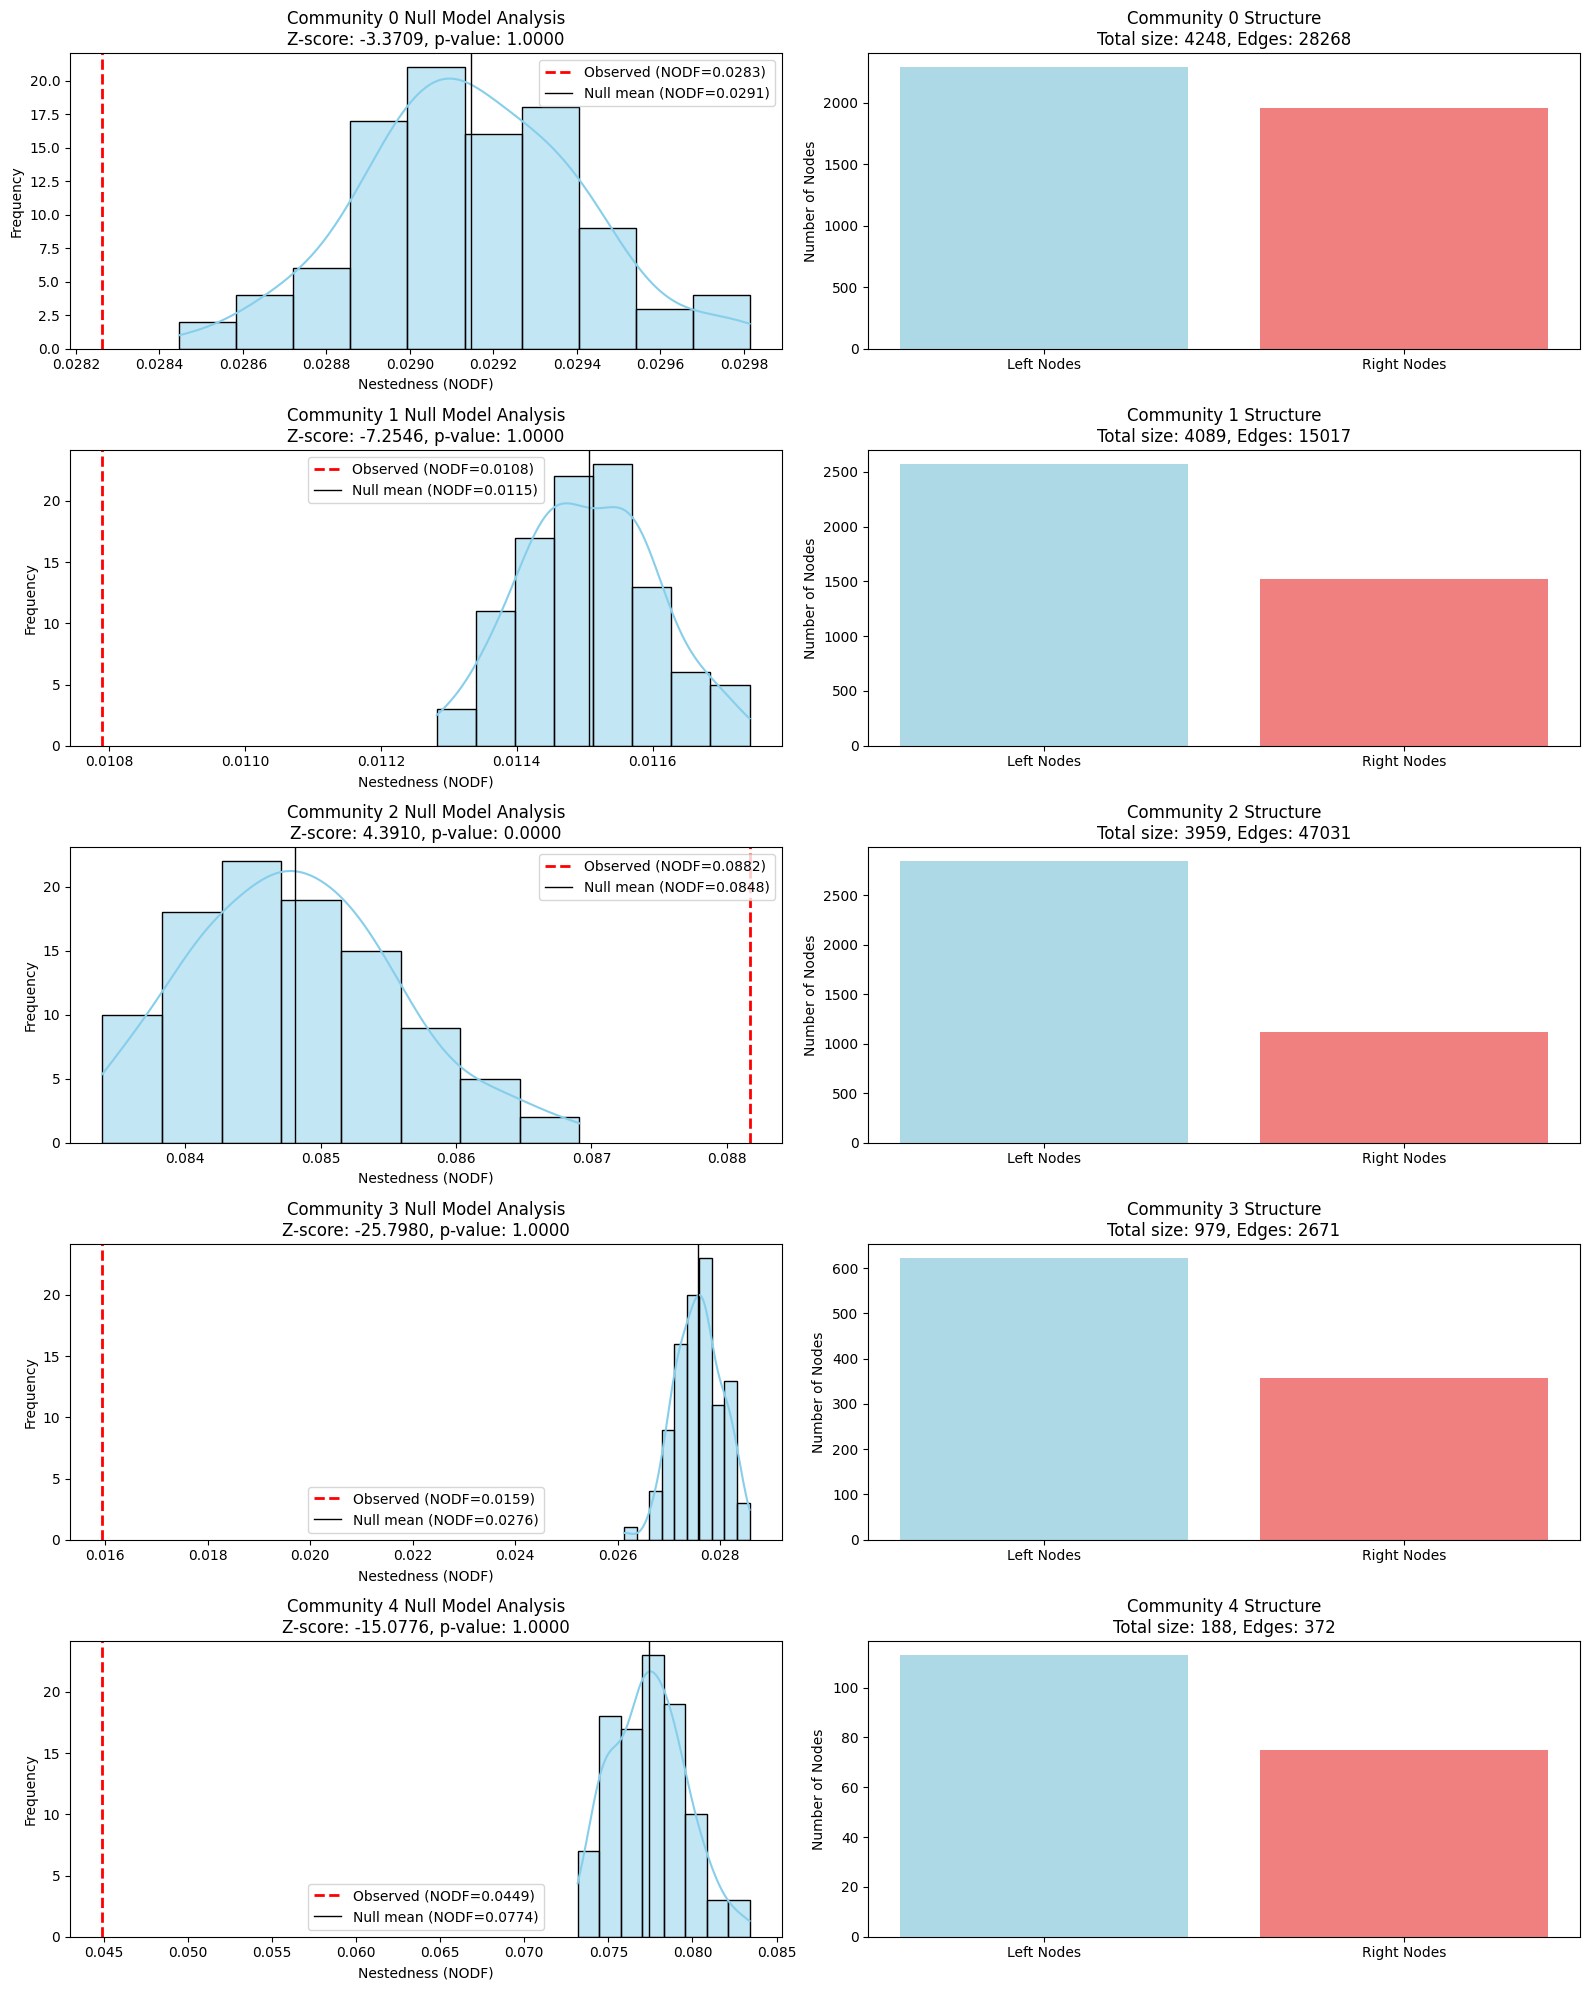
\includegraphics[width=0.8\textwidth]{./assets/null-model-analysis-top-5.png}
\caption{Comparison of observed versus null model nestedness scores for the five largest investor communities. The diagonal line represents equal observed and expected values, with points above the line indicating higher-than-random nestedness. "Left" stands for late stage investors, and "Right" for early stage ones.}
\label{fig:nestedness_comparison}
\end{figure}

\newcommand{\interestingCommunity}{2}
\newcommand{\interestingCommunityNODF}{0.088}
\newcommand{\interestingCommunityPValue}{0.00001}

Community \interestingCommunity{} demonstrates the most pronounced nestedness, exhibiting an NODF score of \interestingCommunityNODF{} with statistical significance of p = \interestingCommunityPValue{}. This community displays a hierarchical investment structure wherein less-connected investors maintain co-investment relationships with a subset of partners associated with highly-connected investors.

\subsection{Community Characterization}

Analysis of the geographic and sectoral characteristics of the most nested communities reveals distinct patterns:

\todo[inline]{Mention only first 3 communities are being compared}

\subsubsection{Geographic Distribution}

Geographic analysis of investor communities reveals distinct spatial clustering patterns that differentiate between early-stage and late-stage investment networks. Figure \ref{fig:geographic_distribution} demonstrates asymmetric geographic distributions across the bipartite network structure.

\todo[inline]{Better format geographic distribution figure}

\begin{figure}[htbp]
\centering
\begin{subfigure}{0.48\textwidth}
    \centering
    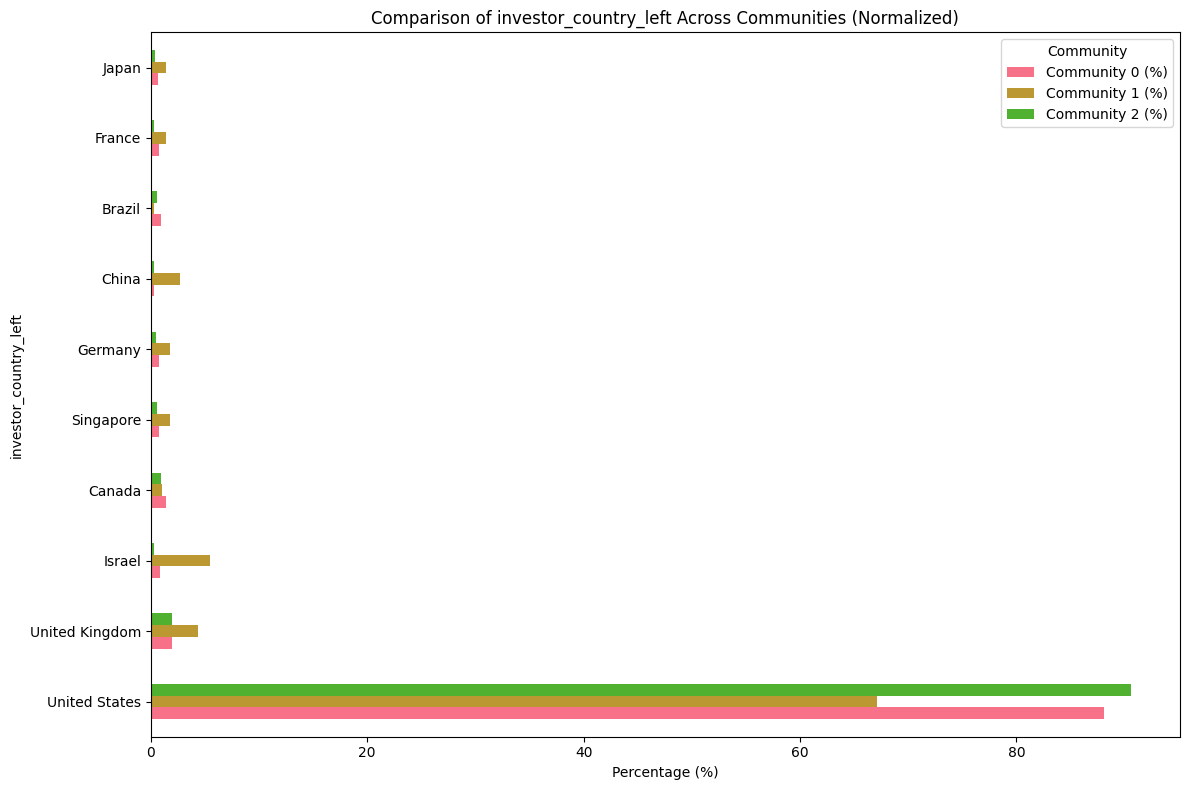
\includegraphics[width=\textwidth]{./assets/investor-left-countries.png}
    \caption{Late-stage investors geographic distribution}
    \label{fig:late_stage_geo}
\end{subfigure}
\hfill
\begin{subfigure}{0.48\textwidth}
    \centering
    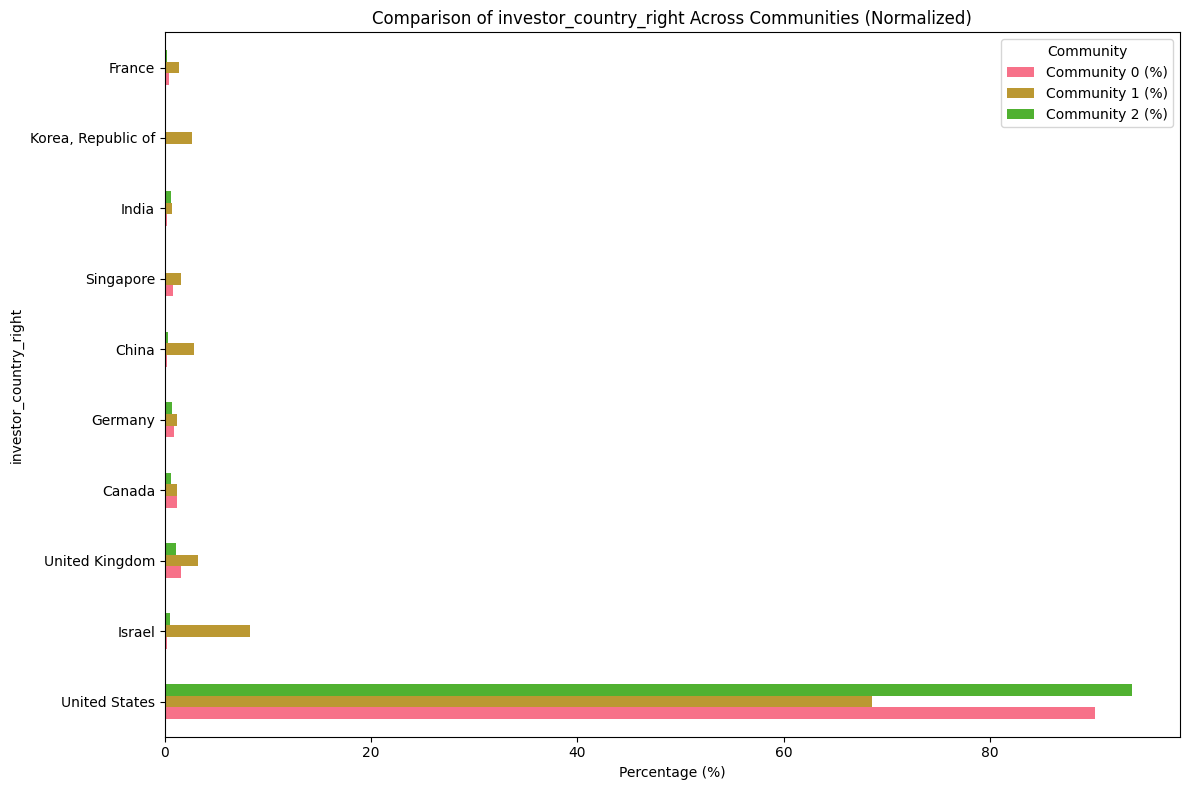
\includegraphics[width=\textwidth]{./assets/investor-right-countries.png}
    \caption{Early-stage investors geographic distribution}
    \label{fig:early_stage_geo}
\end{subfigure}
\caption{Geographic distribution of venture capital investors across the largest communities. The bipartite structure reveals differential geographic clustering between late-stage (left) and early-stage (right) investor networks, with investors from Community \interestingCommunity{} exhibiting greater international diversification.}
\label{fig:geographic_distribution}
\end{figure}

\todo[inline]{Comment geographic distribution}

% The geographic distributions exhibit notable asymmetries: late-stage investors demonstrate greater international representation, while early-stage investors show concentrated domestic clustering. This pattern suggests stage-specific geographic preferences that may reflect risk tolerance, regulatory constraints, or information asymmetries across international markets.

\subsubsection{Investment Stage Preferences}

Investment stage analysis reveals systematic differences in funding round participation across communities. Figure \ref{fig:investment_stage_distribution} demonstrates the distribution patterns of investment types within the bipartite network structure, highlighting distinct preferences between early-stage and late-stage investor groups.

\begin{figure}[htbp]
\centering
\begin{subfigure}{0.48\textwidth}
    \centering
    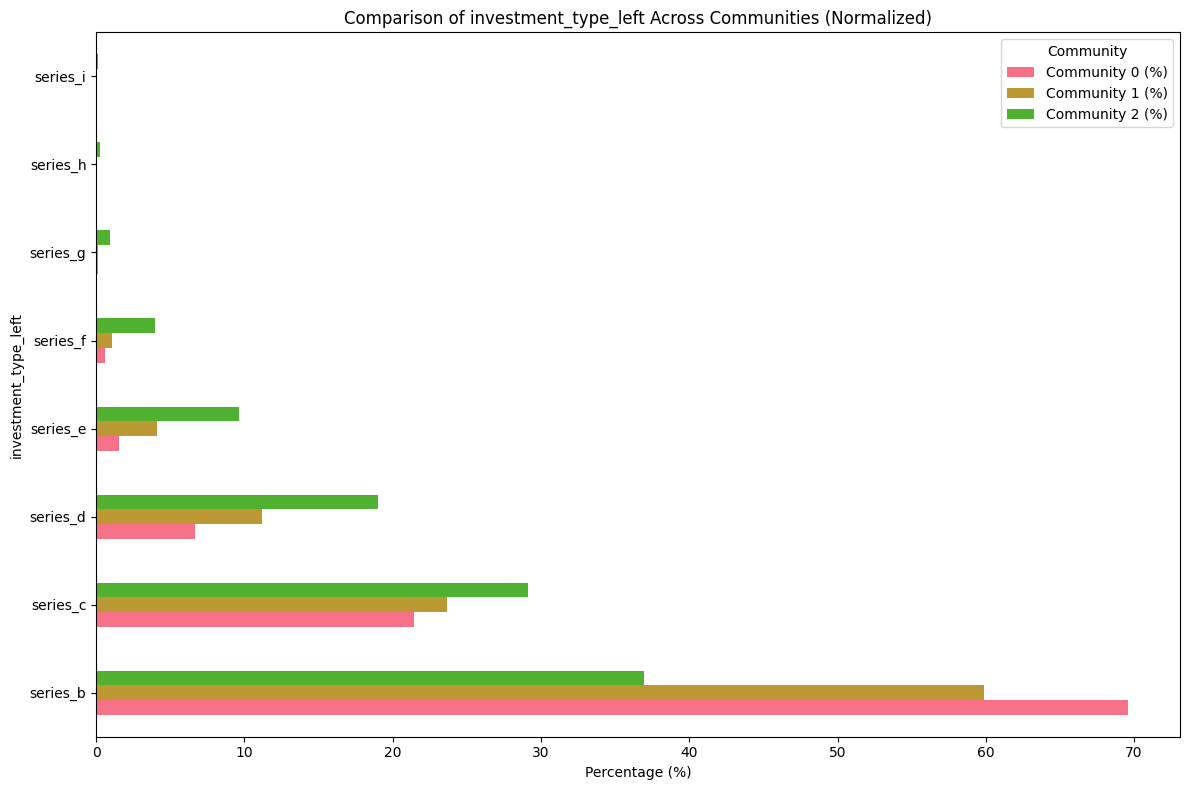
\includegraphics[width=\textwidth]{./assets/late-investment-types-distribution.png}
    \caption{Late-stage investment types distribution}
    \label{fig:late_stage_types}
\end{subfigure}
\hfill
\begin{subfigure}{0.48\textwidth}
    \centering
    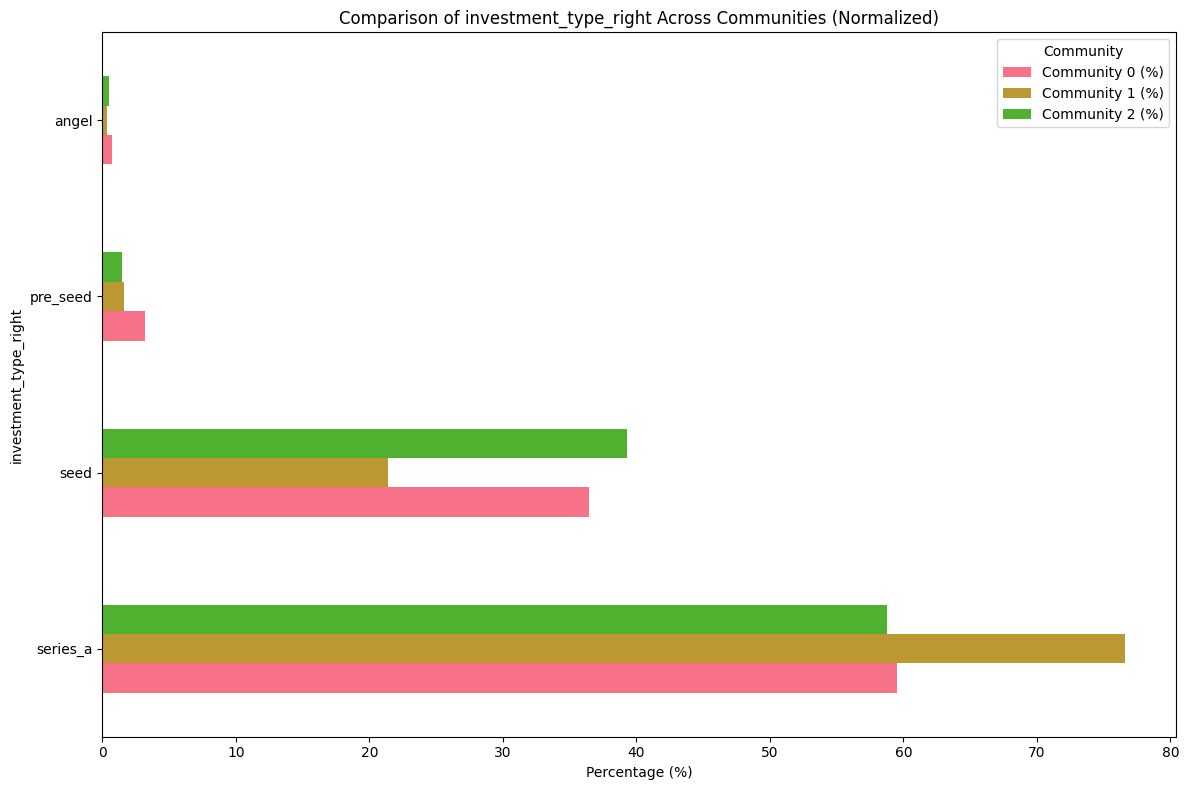
\includegraphics[width=\textwidth]{./assets/early-investment-types-distribution.png}
    \caption{Early-stage investment types distribution}
    \label{fig:early_stage_types}
\end{subfigure}
\caption{Investment stage distribution across the three largest communities. Late-stage investors (left) demonstrate concentration in Series B and later rounds, while early-stage investors (right) exhibit predominant participation in seed and Series A funding rounds. The distribution patterns reveal stage-specific specialization within investor communities.}
\label{fig:investment_stage_distribution}
\end{figure}


\todo[inline]{Comment investment stages distribution}

\subsubsection{Sectoral Focus}

Sectoral analysis reveals distinct industry specialization patterns within nested communities. Figure \ref{fig:sectoral_distribution} illustrates the distribution of investment focus across technology sectors, demonstrating how different communities exhibit varying degrees of sectoral concentration.

\begin{figure}[htbp]
\centering
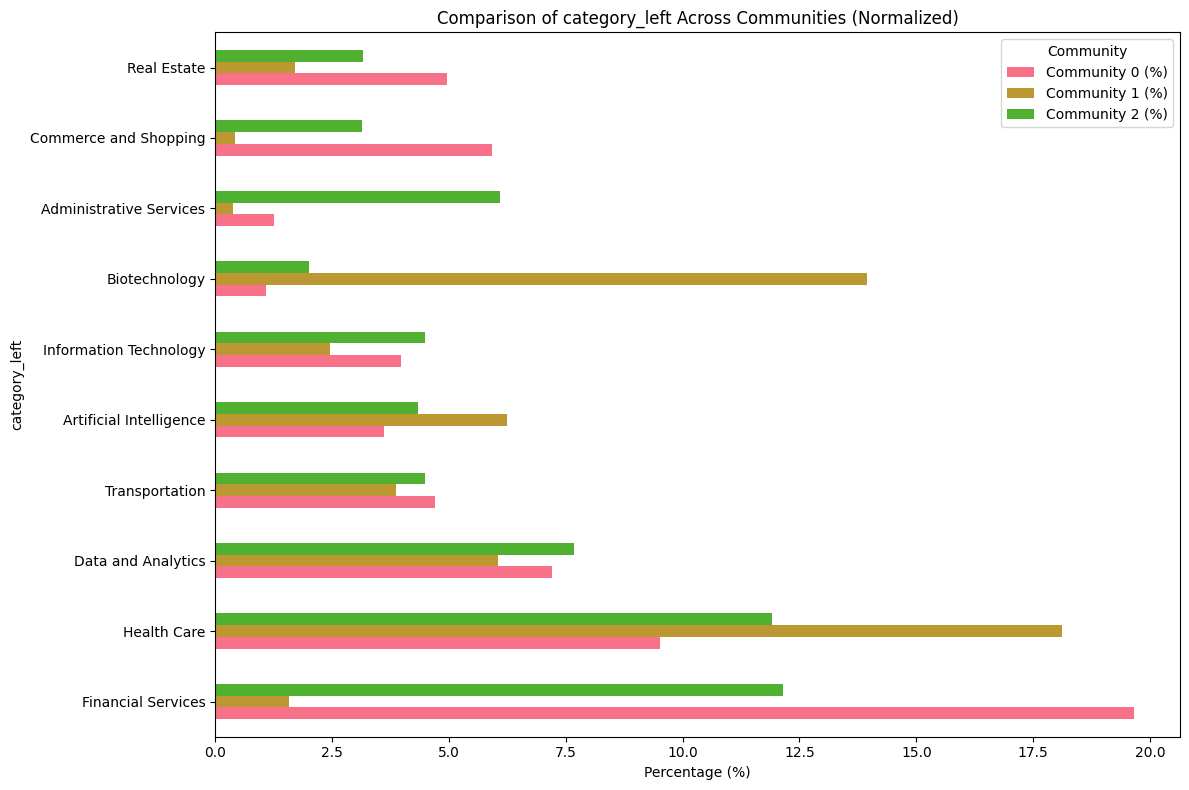
\includegraphics[width=0.8\textwidth]{./assets/sectorial-distribution.png}
\caption{Sectoral distribution across the three largest investor communities. The analysis reveals differential industry focus patterns, with certain communities demonstrating concentrated investment strategies in specific technology sectors while others maintain broader sectoral diversification.}
\label{fig:sectoral_distribution}
\end{figure}

\todo[inline]{Comment sectorial distribution}

% The sectoral concentration patterns indicate that nested communities tend to develop expertise clusters around specific technology domains. This specialization may reflect knowledge spillovers and industry-specific due diligence capabilities that emerge within tightly connected investor groups.

\subsubsection{Funding Characteristics}

Funding analysis demonstrates differential investment patterns within nested communities compared to random network configurations. Figure \ref{fig:funding_characteristics} reveals systematic variations in funding amounts and investment frequency across community structures.

\begin{figure}[htbp]
\centering
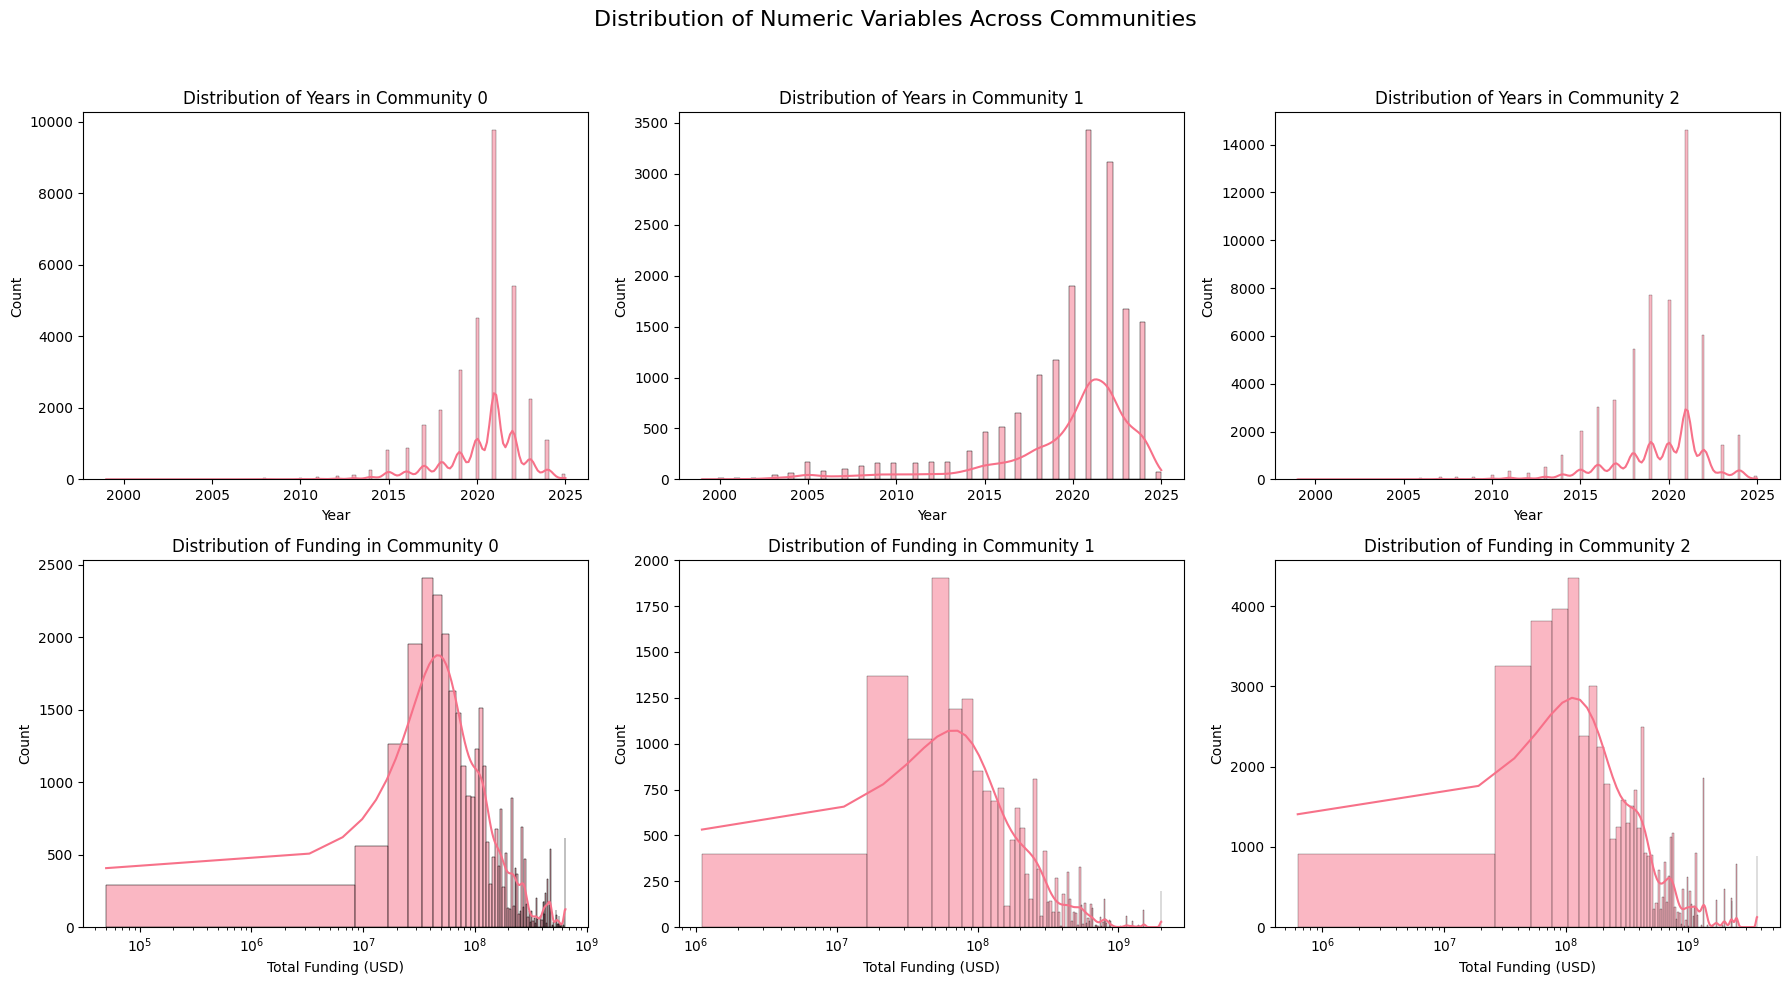
\includegraphics[width=0.8\textwidth]{./assets/funding-characteristics.png}
\caption{Funding characteristics across the three largest investor communities. The analysis reveals systematic differences in investment amounts, round frequency, and funding patterns between communities, with nested structures exhibiting distinct capital deployment strategies compared to randomly organized investor groups.}
\label{fig:funding_characteristics}
\end{figure}

The funding characteristics analysis indicates that nested communities exhibit concentrated capital deployment patterns, with higher-degree investors participating in larger funding rounds while maintaining broader portfolio diversification. This pattern suggests efficient capital allocation mechanisms within hierarchically organized investor networks.


\todo[inline]{Comment more on funding characteristics}

\subsection{Implications and Future Directions}

The discovery of significantly nested communities within the venture capital network has important implications for understanding investor behavior and startup access to capital. The hierarchical structure observed in these communities suggests the existence of informal investment hierarchies that may influence funding accessibility for entrepreneurs.

The presence of nested structures challenges the assumption of random mixing in venture capital markets and suggests that certain investors may serve as "gatekeepers" who influence access to broader investment networks. This finding aligns with social network theories about structural holes and brokerage positions \cite{Borgatti2011}.

The identification of these nested communities opens several avenues for future research into the social and economic mechanisms that drive venture capital ecosystem organization. Understanding these patterns may inform policy discussions about startup ecosystem development and investor network formation.

This analysis provides the foundation for deeper investigation into how nested investor communities influence entrepreneurial ecosystems and capital allocation efficiency, which will be the focus of subsequent research phases.

\todo[inline]{Investigate the economic consequences of nested community structure on startup success rates and funding efficiency.}

\todo[inline]{Analyze the temporal evolution of community nestedness to understand how these structures emerge and persist over time.}

\todo[inline]{Examine whether nested communities provide better or worse outcomes for portfolio companies compared to random investment patterns.}

\todo[inline]{Apply social network theories of structural holes to understand the role of highly connected investors in nested communities.}

\todo[inline]{Investigate whether the nested structure reflects information asymmetries or risk-sharing mechanisms among investors.}

\todo[inline]{Develop theoretical models to explain the emergence of nested structures in investment networks.}

\todo[inline]{Compare nestedness patterns across different geographic markets and time periods to understand generalizability.}

\bibliographystyle{plain}
\bibliography{references}

\end{document}